\documentclass[a4paper,11pt]{style-esi/td}

\usepackage{style-esi/licence}
\usepackage{style-esi/exercice}
\usepackage{style-esi/exemple}
\usepackage{style-esi/question}
\usepackage{style-esi/tutoriel}
\usepackage{style-esi/listing}
\usepackage{style-esi/images}
\usepackage{style-dev1/dev1}

\begin{document}

\seance{1}{Les permissions}
\entete
\titre
\ccbysa{esi-dev1-list@he2b.be}
\lastedit

\bigskip
\tableofcontents

\newpage

%====================
\section{Se documenter}
%=====================


	%====================
	\subsection{Les options}
	%=====================
	
		La plupart des commandes possèdent des \textbf{options}.

		\begin{theorie}{Les options}
			Une \textbf{option modifie le sens} d'une commande ;
			\begin{itemize}
			\item Elle commence par le signe \texttt{-} suivi d'une seule lettre ;
			\item ou encore par le double tiret \texttt{-{}-} suivi d'un nom d'option.
			\item Elle est placée n'importe où après le nom de la commande.   
			\end{itemize}
		\end{theorie}		

		\begin{Experience}{Expérimenter les options}		
			\vspace{-1em}
			\begin{steps}
			\item Tapez la commande \kbd{ls -l}. 
				Vous constatez que le résultat obtenu est beaucoup plus verbeux 
				que celui obtenu sans l'option.
			\item Placez vous dans le dossier \samp{td1} et 
				tapez la commande \kbd{cat -n test}. 
				L'option demande de numéroter les lignes 
			\item Essayez \kbd{cat -{}-number test},
				la version \textit{longue} équivalente à la précédente.
			\end{steps}
		\end{Experience}

	%====================
	\subsection{Recherche d'informations}  
	%====================

		Non seulement, il y a beaucoup de commandes à connaitre mais, en plus, 
		chacune dispose d'une multitude d'options. 
		Impossible de tout retenir ! Comment faire ?   

		\begin{theorie}{Information}
			\begin{itemize}
			\item 
				\kbd{nomCommande -{}-help}
				affiche une aide succincte sur la commande.
			\item 
				\kbd{man nomCommande} affiche une documentation plus complète.
				(\textit{q} pour quitter).
			\end{itemize}
		\end{theorie}

		Si vous ne connaissez pas le nom de la commande,
		consultez les documents que l'on met à votre disposition,
		notamment le \textit{Linux Cheat Sheet}.  

		\begin{Exercice}{Trouver la bonne option} 
			La commande \kbd{ls -l} 
			affiche le contenu du dossier en format \textit{long}.
			La 5\ieme{} colonne donne la taille du fichier (en octets).
			Lorsque les nombres sont grands, ce n'est pas très lisible. 
			Trouvez l'option qui permet d'afficher cette taille sous un format plus lisible.  
			
			\begin{alertbox} 
				De grâce, \textbf{cherchez} la réponse, 
				ne la \textbf{demandez pas} à votre voisin. 
				Le but de cet exercice n'est pas de connaitre l'option 
				(elle n'est pas si utile que \c ca) 
				mais d'apprendre à trouver soi-même l'information.  
			\end{alertbox}
		\end{Exercice}

		\begin{Exercice}{Trouver la bonne commande}
			Quelle commande permet de 
			\begin{itemize}
				\item \textit{nettoyer} l'écran ?  
				\item afficher la date et l'heure ?
			\end{itemize}
		\end{Exercice}

%========================
\section{Les permissions}
%========================

	Comme Linux est un système partagé, il est important de parler de sécurité. 
	Ici, on va se concentrer sur la sécurité au niveau des fichiers 
	et répondre aux questions suivantes :  
	\begin{itemize}
	\item À qui \textbf{appartient} un fichier ?
	\item \textbf{Qui peut faire} quoi avec un fichier ?
	\end{itemize}

	Mais pour commencer il faut d'abord comprendre 
	la notion de \textit{propriétaire}
	et celle de \textit{groupe}. 

	%======================================
	\subsection{Les groupes d'utilisateurs}
	%======================================

		\begin{theorie}{Les groupes}
			Les utilisateurs d'un système Linux sont placés dans des \textbf{groupes}. 
			Un groupe contient un ou plusieurs utilisateur(s) 
			et un utilisateur appartient à un ou plusieurs groupe(s).
		\end{theorie}

		\begin{wrapfigure}{r}{.3\textwidth}
			\vspace{-1em}
			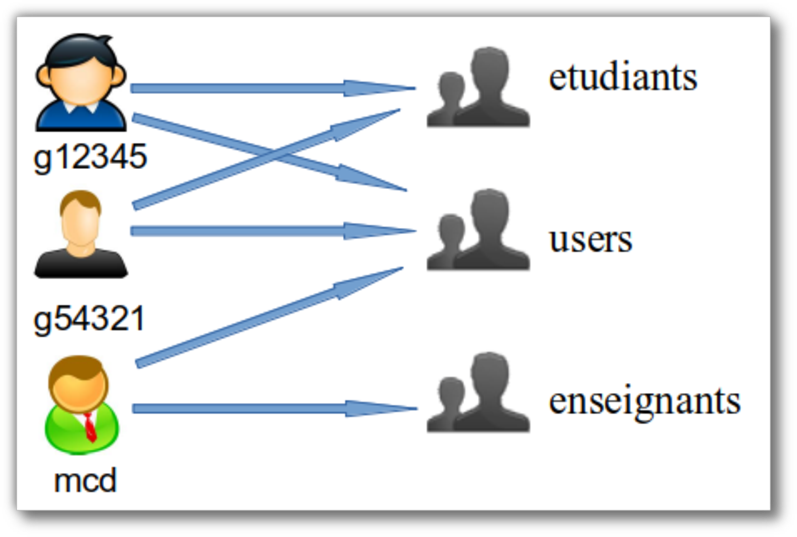
\includegraphics[width=.3\textwidth]{image/groupes.pdf}
			\vspace{-3em}
		\end{wrapfigure}
		\textbf{Exemple} :
		Dans l'exemple ci-contre on peut constater que :
		\begin{itemize}
		\item 
			l'utilisateur \samp{g12345} appartient 
			aux groupes \samp{users} et \samp{etudiants} ;
		\item 
			l'utilisateur \samp{g54321} appartient aux mêmes groupes ;
		\item 
			l'utilisateur \samp{mcd} appartient 
			aux groupes \samp{users} et \samp{enseignants}.
		\end{itemize}
		
		À quoi servent les groupes ? 
		À gérer les permissions. 
		On va pouvoir dire un truc du genre : 
		\og{}Seuls les professeurs peuvent voir le contenu de ce fichier\fg{}.

		\begin{theorie}{Visualiser les groupes}
			La commande \samp{groups} renseigne sur les groupes.
			\begin{itemize}
				\item \kbd{groups} : affiche les groupes de l'utilisateur.
				\item \kbd{groups loginUtilisateur} : affiche les groupes de l'utilisateur donné.
			\end{itemize}
			Le premier groupe de la liste est le \textbf{groupe principal}.
			C'est celui qui sera utilisé par défaut (par exemple, lorsqu'on crée un fichier).
		\end{theorie}

		\begin{Exercice}{Visualiser les groupes}
			\vspace{-1em}
			\begin{itemize}
				\item Visualiser les groupes auxquels vous appartenez.
				\item Quel est votre groupe principal ? 
				\item Quels sont les groupes auxquels appartient votre professeur ?
				\item Avez-vous un groupe en commun avec lui ?
				\item Quel(s) groupe(s) Linux avez-vous en commun avec les autres étudiants de votre groupe ÉSI ?
			\end{itemize}
		\end{Exercice}

		\begin{colxbox}[colback=white,drop fuzzy shadow]
			Les groupes qui existent concrètement sur une machine sont définis 
			par l'administrateur%
			\footnote{
				L'administrateur est la personne qui installe 
				un système d'exploitation et le gère au quotidien : 
				installation de logiciels, 
				gestion des comptes utilisateurs et des groupes, 
				sauvegardes, gestion des panne\dots{}
				Sur Linux, on dit aussi le « super user », 
				le « compte root » ou le « root ».
			} de la machine. 		
			Sur \texttt{linux1}, 
			il y a 3 groupes pour les utilisateurs.
			\begin{itemize}
				\item \textbf{\samp{users}} : tous les utilisateurs sont dans ce groupe
				\item \textbf{\samp{etudiants}} : tous les étudiants sont dans ce groupe
				\item \textbf{\samp{enseignants}} : tous les professeurs sont dans ce groupe	
			\end{itemize}
		\end{colxbox}

		\medskip
		\begin{alertbox}
			Attention, on remarque que vous confondez souvent 
			la notion de \textbf{groupe d'étudiants} à l'école
			et les \textbf{groupes sur Linux}.
			C'est un même mot qui recouvre 2 
			\textbf{concepts} complètement \textbf{différents}.
		\end{alertbox}

	%======================================
	\subsection{Propriétaire d'un fichier}
	%======================================
	
		\exergue{La propriété est un piège: ce que nous croyons posséder nous possède.}
			{Alphonse Karr}
		\vspace{2em}

		\exergue{La propriété c'est le vol.}{Pierre Joseph Proudhon}
		\vspace{1em}

		\begin{theorie}{Propriétaire}
			Chaque fichier/dossier \textbf{appartient} à une personne, 
			son \textbf{propriétaire}.
			On peut le visualiser via la commande \kbd{ls -l}.
		\end{theorie}

		\begin{center}
			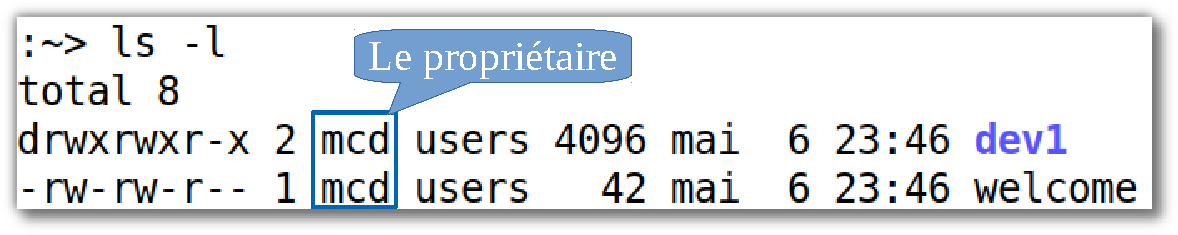
\includegraphics[height=4em]{image/owner}
		\end{center}

		\begin{Exercice}{Propriétaire}
			Visualisez le propriétaire des fichiers de votre dossier personnel.
		\end{Exercice}

	%======================================
	\subsection{Groupes d'un fichier}
	%======================================

	

\begin{Tutoriel}{Groupe}	
%					\textcolor{white}{.} \par
%
%\par
\begin{enumerate}
	
	\item Visualisez vos fichiers et déterminez à quel groupe ils appartiennent.
	\item Créez un fichier de test et modifiez le groupe auquel il appartient.
\end{enumerate}
		\end{Tutoriel}


		\subparagraph{FAQ} 

%\textcolor{white}{.} \par
%\par
\textbf{Les fichiers dans mon dossier personnel ne sont pas automatiquement à moi ?}
%\par

Non. En pratique c'est généralement le cas, 
mais on peut très bien trouver dans un dossier personnel un fichier qui appartient à quelqu'un d'autre.  

%\par

        \subsection{Les permissions}  
à présent que vous savez qu'un fichier a un propriétaire et appartient à un groupe, 
on peut étudier la notion de permission.    

%\par
\textbf{Restez concentré} ! 
Cette partie est plus longue et un peu plus difficile que ce que vous avez déjà appris 
mais c'est absolument nécessaire pour la suite.   
%\par

Un retour vers les points 17 à 19 du guide visuel sera peut-\^etre encore nécessaire...  

%\par

\begin{Exercice}{Déterminez les bonnes permissions}
	
	Remplissez les blancs avec la permission correcte (r, w, x ou -).  Il s'agit
	de trouver la permission minimale à mettre pour répondre à la demande.   
	
	\begin{itemize}
		
		\item Pour un fichier Java, la permission la plus adéquate est
			\textcolor{gray}{\underline{\hspace*{1em}}}
			\textcolor{gray}{\underline{\hspace*{1em}}}
			\textcolor{gray}{\underline{\hspace*{1em}}} 
	
		\item Le fichier qui contient (l'exécutable de) \texttt{ls}
			a probablement comme permisson\\
		\textcolor{gray}{\underline{\hspace*{1em}}}
		\textcolor{gray}{\underline{\hspace*{1em}}}
		\textcolor{gray}{\underline{\hspace*{1em}}}

		    Vous pouvez le vérifier. Comment ? 
	
\end{itemize}
	
\end{Exercice}

\begin{Exercice}{Exercice}
		%				\textcolor{white}{.} \par
%	\par
	Soit le fichier "Max.java" de la capture d'écran ci-dessous.  
	%\par
	\begin{figure}[hbt]
		\begin{center}
			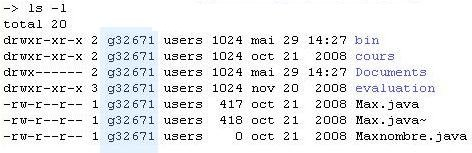
\includegraphics[width=0.8\linewidth,height=0.8\textheight,keepaspectratio=true]{image/ls-l.jpg}
			
		\end{center}
		
		\caption[Contenu détaillé d'un dossier]{Contenu détaillé d'un dossier}
	\end{figure}
	
	Est-ce qu'un professeur peut l'éditer ? 
	
%	\par
	%\fcolorbox{gray}{verylightgray}{\parbox{\textwidth}{\textcolor{verylightgray}{\LARGE  Non ! Le droit d'écriture n'est accordé qu'au propriétaire.  }}} {\footnotesize\emph{}\par} 
	%(la réponse est disponible dans la version en ligne)
\end{Exercice}	

	
\begin{Exercice}{Déterminez les bonnes permissions}	
	           %     \textcolor{white}{.} %\par	
	Soit le fichier "Max.java" de la capture d'écran ci-dessus.
	
	On voudrait que l'étudiant g32671 puisse travailler  
	normalement, que les autres étudiants ne puissent pas tricher sur  
	lui mais que les professeurs puissent lire son travail.   
	
	\begin{itemize}
		
		\item 
		Quel groupe faut-il donner au fichier ?
		\par
		\textcolor{gray}{\underline{\hspace*{10em}}} 
		\item 
		Quelle commande permet de donner ce groupe au fichier ?
		\par
		\textcolor{gray}{\underline{\hspace*{3em}}}  \textcolor{gray}{\underline{\hspace*{10em}}}  \textcolor{gray}{\underline{\hspace*{10em}}} 
		\item 
		Quelles permissions minimales donner au fichier ?                
		\par
		\textcolor{gray}{\underline{\hspace*{1em}}}  \textcolor{gray}{\underline{\hspace*{1em}}}  \textcolor{gray}{\underline{\hspace*{1em}}}  \textcolor{gray}{\underline{\hspace*{1em}}}  \textcolor{gray}{\underline{\hspace*{1em}}}  \textcolor{gray}{\underline{\hspace*{1em}}}  \textcolor{gray}{\underline{\hspace*{1em}}}  \textcolor{gray}{\underline{\hspace*{1em}}}  \textcolor{gray}{\underline{\hspace*{1em}}} 
		\item 
		Quelle commande permet de donner ces permissions au fichier ?
		\par
		\textcolor{gray}{\underline{\hspace*{3em}}}  \textcolor{gray}{\underline{\hspace*{2em}}}  \textcolor{gray}{\underline{\hspace*{10em}}} 
	\end{itemize}
	
	
\end{Exercice}


\begin{Exercice}{} 
	Reprenez les permissions affichées dans la capture d'écran ci-dessous 
et exprimez-les avec un nombre de 3 chiffres.  

\par
\begin{figure}[hbt]
	\begin{center}
		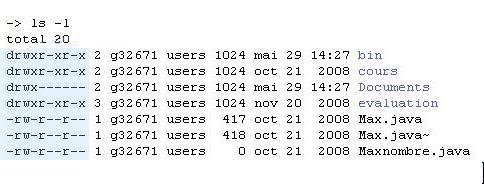
\includegraphics[width=0.8\linewidth,height=0.8\textheight,keepaspectratio=true]{image/ls-l-permissions.jpg}
		
	\end{center}
	
	\caption[Contenu détaillé d'un dossier]{Contenu détaillé d'un dossier}
\end{figure}
\end{Exercice}
		
		
\begin{Tutoriel}{Permissions par défaut} 	
	%	\textcolor{white}{.} \par
		
	%	\par	
		\begin{enumerate}
			
			\item Si ce n'est pas encore fait, créez un dossier "td2".
			\item Créez-y un fichier vide.
			\item Demandez les détails du fichier (propriétaire, groupe, permission)
		\end{enumerate}
		
		On constate qu'un nouveau fichier appartient à celui qui l'a créé 
		(on s'en doute) et au groupe principal du créateur. 
		Il y a aussi des permissions par défaut (plut\^ot permissives dans notre cas).  
		
		\par
\end{Tutoriel}		
		
		\subparagraph{Modifier les permissions} 

\textcolor{white}{.} \par

\par

Vous savez que la commande qui permet de modifier les permissions d'un fichier est 
\,\verb|chmod|\,.  

\par

Prenez le temps de \textbf{lire} 
la page de \textbf{manuel} de cette commande.   

\par
	
	\begin{Tutoriel}{Modifier les permissions} 
\begin{enumerate}	
	\item Créez un fichier "brol" dans le dossier "td2" avec quelques mots.
	\item Faites en sorte que personne d'autre ne puisse en voir le contenu.
	\item Faites en sorte que tout le monde puisse voir son contenu mais pas le modifier. 
	\item 
	Faites en sorte que les autres étudiants ne puissent pas voir son contenu mais les professeurs bien. 
	Attention, pour ce faire, il faut pouvoir distinguer les étudiants des enseignants; et donc, distinguer les groupes.
	
\end{enumerate}
		
	\end{Tutoriel}

	\begin{Tutoriel}{Modifier encore les permissions}           
Modifiez les droits de votre dossier "td2" et, si nécessaire, 
des fichiers qui s'y trouvent pour que tout le monde puisse  
%\par
\begin{enumerate}
	
	\item voir quels fichiers s'y trouvent mais sans pouvoir lire le contenu de ces fichiers;
	\item modifier le contenu d'un des fichiers mais pas supprimer ce fichier;
	\item supprimer un fichier mais pas modifier son contenu.
\end{enumerate}
	
\end{Tutoriel}


		\subparagraph{FAQ} 

\textcolor{white}{.} \par

\par
\textbf{Pourquoi avoir choisi 4, 2 et 1 pour désigner les permissions ?}
\par

C'est lié au code binaire. 'rwx' donne, pour 'r', la valeur '100' soit 4 en décimal.  

\par
\textbf{Vous dites que dans un affichage en format long, 
	le premier caractère indique si c'est un fichier simple ('-') ou un dossier ('d'). 
	Pourtant j'ai déjà vu d'autres symboles. C'était quoi ?
}
\par

Il existe d'autres types de fichiers que les deux que nous avons vus. 
Ils se rencontrent moins souvent et sont surtout utilisés par le système.
Par exemple, certains définissent des \textit{pilotes} vers le matériel. 
Si vous voulez en savoir plus, vous pouvez lire
ceci (\url{en.wikipedia.org/wiki/Unix\_file\_types}).  

\par
\textbf{Vous avez mentionné les permissions 'r', 'w' et 'x'. 
	Pourtant j'ai déjà vu d'autres lettres dans la zone réservée aux permissions. 
	C'était quoi ?
}
\par

Il y a 3 permissions dont nous n'avons pas parlé parce qu'elles sont moins courantes : 
le \textit{suid} (set user id), 
le \textit{sgid} (set group id) 
et le \textit{sticky}. 
Si vous voulez en savoir plus, vous pouvez lire   
ceci (\url{fr.wikipedia.org/wiki/Permissions\_UNIX}).  

\par
\textbf{Vous n'avez pas expliqué le sens de la 2\textsuperscript{e} colonne 
	fournie par la commande ls (juste avant le propriétaire) ?
}
\par

C'est vrai mais c'est moins utile et plus lié à la structure interne du système de fichier. 
Je veux bien vous dire qu'il s'agit du nombre de liens physiques sur le fichier 
mais je sens que vous commencez déjà à regretter d'avoir posé la question ;)  

\par
\textbf{Nous avons vu qu'un fichier est créé avec des permissions par défaut. 
	C'est configurable ?
}
\par

Oui. Voyez la commande \,\verb|umask|\,.  

\par


        \subsection{Conclusion}

\subparagraph{FAQ} 

\textcolor{white}{.} %\par

\par
\textbf{Euh ! Je n'ai pas fini. C'est normal ?}
%\par
Non, c'est que vous avez mal préparé votre TD avant de venir au labo. 
Terminez-le en remédiation et/ou à la maison car la semaine prochaine, 
nous en attaquons un nouveau et, cette fois, essayez de mieux vous y préparer!  

\par
\textbf{Je n'ai pas Linux à la maison. Je peux quand m\^eme terminer mon TD ?}
\par

Non. Vous devrez rapidement disposer d'un Linux fonctionnel à la maison.
Ce qui devrait d'ailleurs \^etre le cas si vous avez fait
les exercices demandés au cours d'introduction à l'OS.

\par
\textbf{J'ai un Linux à la maison et les groupes ne sont pas les m\^emes. C'est normal ?}
\par

Oui. 
Les groupes dépendent à la fois de la distribution particulière utilisée
et de la fa\c con dont l'administrateur (le root) a configuré le système.   

\par

\end{document}

	
